\documentclass[../relazione.tex]{subfiles}

\begin{document}
\section{Analisi dell'utenza}
		Quando si parla di utenza l'attenzione si sposta sull'interfaccia: come il sito appare all'utente ma anche come l'utente interagisce con esso.\\
		Essendo il sito web di un ristorante si può supporre che una qualsiasi persona sia interessata ad informarsi sul ristorante o ordinare take away, per questo motivo è fondamentale l'accessibilità del sito.\\\\
		Una grossa fetta di utenti è composta dai ragazzi più giovani, molti di cui sono assolutamente innamorati della cucina giapponese e tendono a frequentare il ristorante oppure ordinare take away.
		Per questo motivo il gruppo ha deciso di definire lo stile del sito anche per i dispositivi mobile, tenendo conto che la maggior parte degli accessi al sito da parte di ragazzi giovani verrà effettuata da smartphone o tablet.
		\begin{figure}[H]
			\centering
			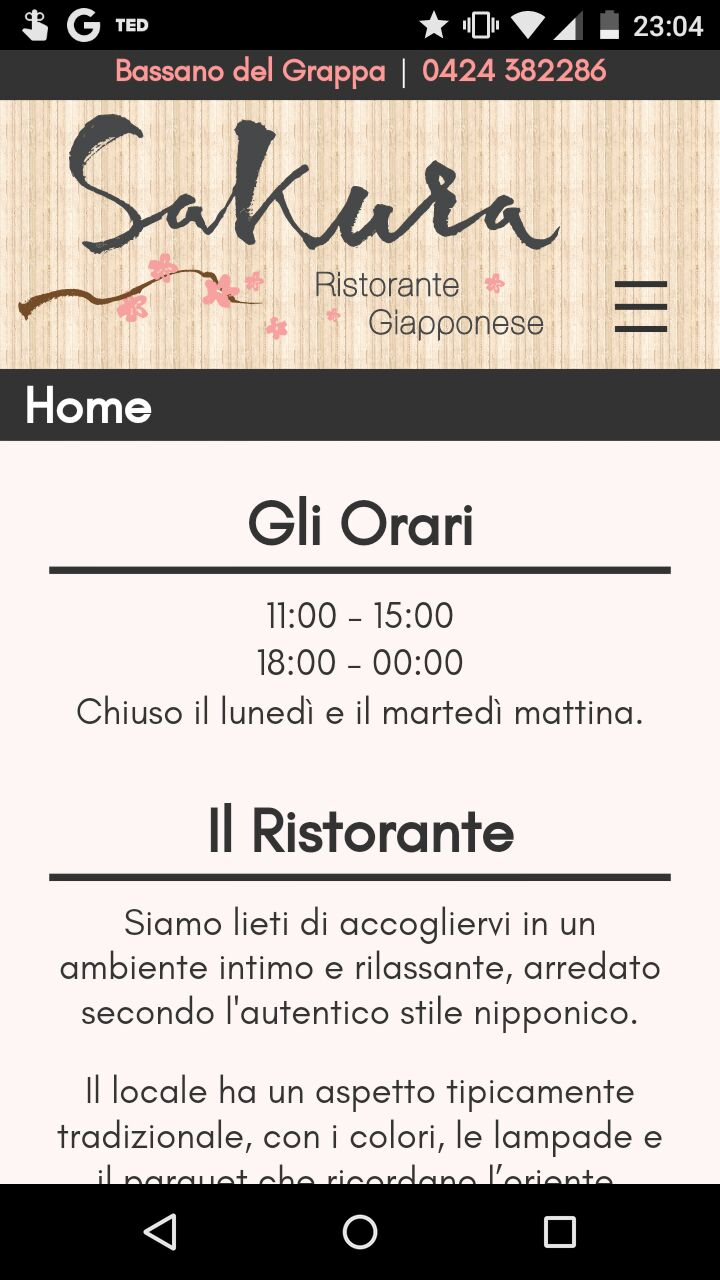
\includegraphics[scale=0.15]{images/mobile1}
			\caption{Esempio di pagina vista da dispositivo mobile}
			\label{fig:Esempio di pagina vista da dispositivo mobile}
		\end{figure}
		Questi dati sono stati ricavati dall'esperienza personale di alcuni membri del gruppo ma anche da un confronto con lo stesso proprietario del ristorante Sakura: egli infatti ci ha dato molte informazioni interessanti riguardo il mondo della cucina giapponese che abbiamo deciso di sfruttare a nostro vantaggio per ottenere un sito \textit{giusto} per il suo bacino d'utenza.\\\\
		La parte di amministrazione del sito ha un utenza limitata al gestore del ristorante, quindi l'utente che utilizzerà l'area amministratore sarà un utente che ha conoscenze di \texttt{XHTML}.\\
		Per questa sezione è stato mantenuto lo stesso stile, ma per ovvi motivi non si è puntato fortemente il dito sull'estetica così come è stato fatto per la restante parte. 
\end{document}